\subsection{Naive beginnings}
We start by modelling the states of the agents:

\begin{HaskellCode}
data SIRState = Susceptible | Infected | Recovered
\end{HaskellCode}

Agents are ill for some duration, meaning we need to keep track when a potentially infected agent recovers. Also a simulation is stepped in discrete or continuous time-steps thus we introduce a notion of \textit{time} and $\Delta t$ by defining:

\begin{HaskellCode}
type Time      = Double
type TimeDelta = Double
\end{HaskellCode}

Now we can represent every agent simply as a tuple of its SIR state and its potential recovery time. We hold all our agents in a list:
\begin{HaskellCode}
type SIRAgent = (SIRState, Time)
type Agents   = [SIRAgent]
\end{HaskellCode}

Next we need to think about how to actually step our simulation. For this we define a function which advances our simulation with a fixed $\Delta t$ until a given time $t$ where in each step the agents are processed and the output is fed back into the next step. This is the source of pro-activity as agents are executed in every time step and can thus initiate actions based on the passing of time.
As already mentioned, the agent-based implementation of the SIR model is inherently stochastic which means we need access to a random-number generator. We decided to use the Random Monad at this point as threading a generator through the simulation and the agents could become very cumbersome. Thus our simulation stepping runs in the Random Monad:

\begin{HaskellCode}
runSimulation :: RandomGen g 
  => Time -> TimeDelta -> Agents -> Rand g [Agents]
runSimulation tEnd dt as = runSimulationAux 0 as []
  where
    runSimulationAux :: RandomGen g 
      => Time -> Agents -> [Agents] -> Rand g [Agents]
    runSimulationAux t as acc
      | t >= tEnd = return (reverse (as : acc))
      | otherwise = do
        as' <- stepSimulation dt as 
        runSimulationAux (t + dt) as' (as : acc)

stepSimulation :: RandomGen g 
  => TimeDelta -> Agents -> Rand g Agents
stepSimulation dt as = mapM (runAgent dt as) as
\end{HaskellCode}

Now we can implement the behaviour of an individual agent. First we need to distinguish between the agents SIR states:

\begin{HaskellCode}
runAgent :: RandomGen g 
  => TimeDelta -> Agents -> SIRAgent -> Rand g SIRAgent
runAgent _  as   (Susceptible, _) = susceptibleAgent as
runAgent dt _  a@(Infected   , _) = return (infectedAgent dt a)
runAgent _  _  a@(Recovered  , _) = return a
\end{HaskellCode}

An agent gets fed the states of all agents in the system from the previous time-step so it can draw random contacts - this is one, very naive way of implementing the interactions between agents.

From our implementation it becomes apparent that only the behaviour of a susceptible agent involves randomness and that a recovered agent is simply a sink - it does nothing and stays constant.

Lets look how we can implement the behaviour of a susceptible agent. It simply makes contact on average with a number of other agents and gets infected with a given probability if an agent it has contact with is infected.
When the agent gets infected it calculates also its time of recovery by drawing a random number from the exponential distribution meaning it is ill on average for \textit{illnessDuration}.

\begin{HaskellCode}
susceptibleAgent :: RandomGen g => Agents -> Rand g SIRAgent
susceptibleAgent as = do
    -- draws from exponential distribution
    rc <- randomExpM (1 / contactRate) 
    cs <- forM [1..floor rc] (const (makeContact as))
    if elem True cs
      then infect
      else return (Susceptible, 0)
  where
    makeContact :: RandomGen g => Agents -> Rand g Bool
    makeContact as = do
      randContact <- randomElem as
      case fst randContact of
        -- returns True with given probability 
        Infected -> randomBoolM infectivity 
        _        -> return False

    infect :: RandomGen g => Rand g SIRAgent
    infect = randomExpM (1 / illnessDuration) 
               >>= \rd -> return (Infected, rd)
\end{HaskellCode}

The infected agent is trivial. It simply recovers after the given illness duration which is implemented as follows:

\begin{HaskellCode}
infectedAgent :: TimeDelta -> SIRAgent -> SIRAgent
infectedAgent dt (_, t) 
    | t' <= 0   = (Recovered, 0)
    | otherwise = (Infected, t')
  where
    t' = t - dt  
\end{HaskellCode}

\subsubsection{Results}
When running our naive implementation with increasing population sizes we get the dynamics as seen in Figure \ref{fig:sir_abs_dynamics_naive}. With increasing number of agents \cite{macal_agent-based_2010} our solution becomes increasingly smoother and approaches the SD dynamics from Figure \ref{fig:sir_sd_dynamics}  but doesn't quite match them because we are under-sampling the contact-rate. We will will address this problem in the next section.

\begin{figure}
\begin{center}
	\begin{tabular}{c c}
		\begin{subfigure}[b]{0.22\textwidth}
			\centering
			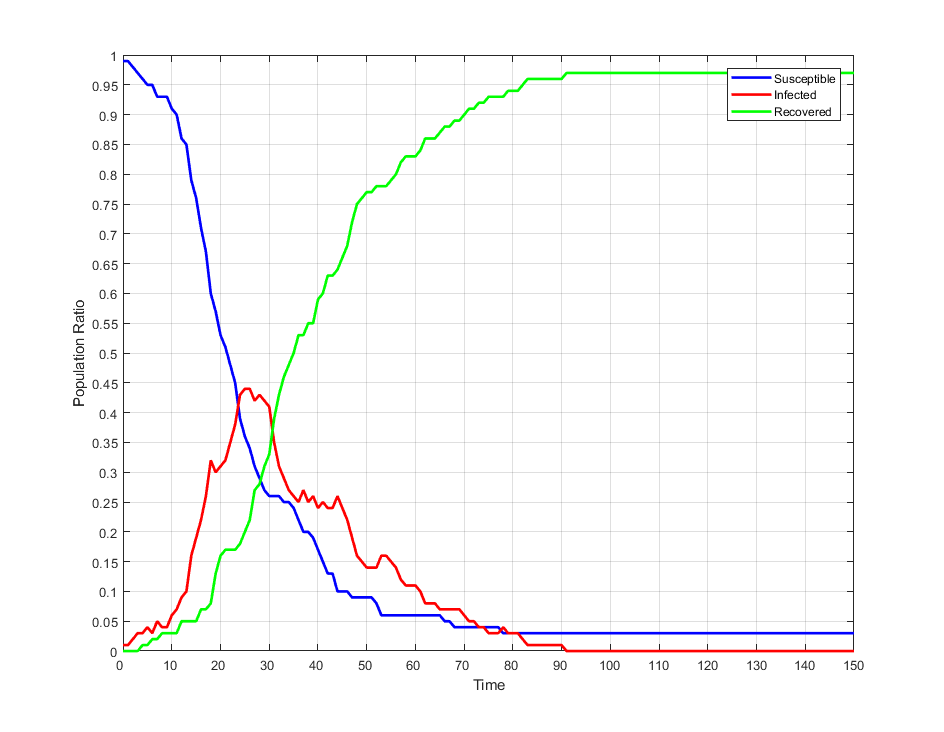
\includegraphics[width=1.0\textwidth, angle=0]{./fig/step1_randmonad/SIR_100agents_150t_1dt.png}
			\caption{100 Agents}
			\label{fig:sir_abs_approximating_1dt_100agents}
		\end{subfigure}
    	
    	&
    	
		\begin{subfigure}[b]{0.20\textwidth}
			\centering
			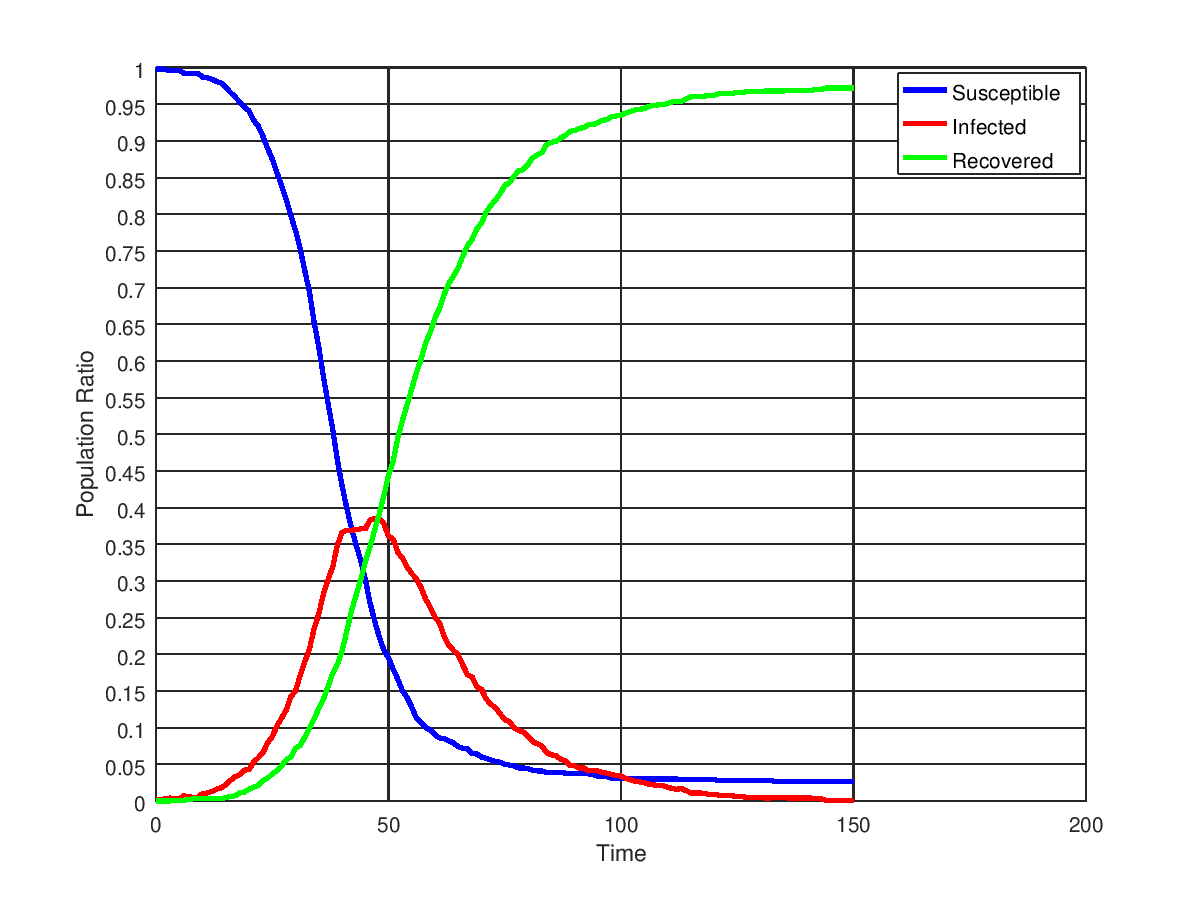
\includegraphics[width=1.0\textwidth, angle=0]{./fig/step1_randmonad/SIR_1000agents_150t_1dt.png}
			\caption{1,000 Agents}
			\label{fig:sir_abs_approximating_1dt_1000agents}
		\end{subfigure}
	\end{tabular}
	
	\caption{Naive simulation of SIR using the agent-based approach. Varying population size, contact rate $\beta = \frac{1}{5}$, infection probability $\gamma = 0.05$, illness duration $\delta = 15$ with initially 1 infected agent. Simulation run for 150 time-steps with fixed $\Delta t = 1.0$.} 
	\label{fig:sir_abs_dynamics_naive}
\end{center}
\end{figure}

\subsubsection{Discussion}
Reflecting on our first naive approach we can conclude that it already introduced most of the fundamental concepts of ABS
\begin{itemize}
	\item Time - the simulation occurs over virtual time which is modelled explicitly divided into \textit{fixed} $\Delta t$ where at each step all agents are executed.
	\item Agents - we implement each agent as an individual, with the behaviour depending on its state.
	\item Feedback - the output state of the agent in the current time-step $t$ is the input state for the next time-step $t + \Delta t$.
	\item Environment - as environment we implicitly assume a fully-connected network (complete graph) where every agent 'knows' every other agents, including itself and thus can make contact with all of them.
	\item Stochasticity - it is an inherently stochastic simulation, which is indicated by the Random Monad type and the usage of \textit{randomBoolM} and \textit{randomExpM}.
	\item Deterministic - repeated runs with the same initial random-number generator result in same dynamics. This may not come as a surprise but in Haskell we can guarantee that property statically already at compile time because our simulation runs in the Random Monad and \textit{not} in the IO Monad. This guarantees that no external, uncontrollable sources of randomness can interfere with the simulation.
	\item Dynamics - with increasing number of agents the dynamics smooth out \cite{macal_agent-based_2010}.
\end{itemize}

Nonetheless our approach has also weaknesses and dangers:
\begin{enumerate}
	\item $\Delta t$ is passed explicitly as argument to the agent and needs to be dealt with explicitly. This is not very elegant and a potential source of errors - can we do better and find a more elegant solution? 
	\item The way our agents are represented is not very modular. The state of the agent is explicitly encoded in an ADT and when processing the agent, the function needs always first distinguish between the states. Can we express it in a more modular way e.g. continuations?
\end{enumerate}

We now move on to the next section in which we will address these points and the under-sampling issue.